\documentclass[10pt,conference]{IEEEtran}

\usepackage{graphicx}
\usepackage{amsmath}
\usepackage{booktabs}
\usepackage{array}
\usepackage[table]{xcolor}
\usepackage{hyperref}
\usepackage{float}
\usepackage{placeins}

\hypersetup{colorlinks=true, linkcolor=blue, citecolor=blue, urlcolor=blue}
\renewcommand{\arraystretch}{1.1}

\begin{document}

\title{Bit\'acora de Dise\~no\\ Cerradura Electr\'onica}

\author{
\IEEEauthorblockN{Jose Andr\'es Chavarr\'ia Gamboa}
\IEEEauthorblockN{Isaac Andr\'es Arias Picado}
\IEEEauthorblockA{Escuela de Ingenier\'ia en Computadores, Instituto Tecnol\'ogico de Costa Rica (TEC)\\
CE--1107 Fundamentos de Arquitectura de Computadores --- Profesor: Luis Alberto Chavarr\'ia Zamora}
}

\maketitle

\section{2 de septiembre}
\textbf{Objetivo:} el d\'ia de hoy se busca iniciar con la planeaci\'on del dise\~no general del
sistema de cerradura con clave. Se toman decisiones de dise\~no sobre el modelo y se analiza el
funcionamiento de cada bloque por separado.

Se repas\'o el enunciado del proyecto y se defini\'o c\'omo se iba a resolver cada bloque del
diagrama general (sensores $\rightarrow$ circuito combinacional $\rightarrow$ BCD $\rightarrow$
display de 7 segmentos, m\'as la rama de desacople/accionador). Las decisiones principales:

\begin{itemize}
\item Por ahora el sistema es completamente combinacional, sin ning\'un elemento de memoria: los 3
d\'igitos de la contrase\~na se fijan directo con dos bancos de DIP-switch, y esa combinaci\'on
entra directo a las compuertas del comparador, que a su vez alimentan al decodificador de 7
segmentos.
\item Se fija como contrase\~na de prueba \texttt{512} para cerrar y \texttt{450} para abrir.
\item Se trabaja \'unicamente con compuertas CMOS (serie 74HC) en todo el circuito, sin mezclar con
TTL: la CMOS tiene una impedancia de entrada much\'isimo m\'as alta, un rango de voltaje de
alimentaci\'on distinto y m\'argenes de ruido distintos a los de TTL, as\'i que una salida de una
familia no necesariamente entrega el nivel que la otra reconoce como v\'alido. Adem\'as, toda
entrada CMOS que no se vaya a usar se debe poner en GND, esto para evitar fallos en el dispositivo por el ruido generado al dejar la entrada al aire. Si en alguna etapa hiciera
falta interconectar con otra familia, se documentar\'a el uso de un traductor de niveles.
\item Cada etapa se dise\~na primero como tabla de verdad, se reduce con mapas K y/o l\'ogica booleana y se simula antes
de armar en protoboard.
\item El dise\~no del sistema, las decisiones de arquitectura y todas las tablas de verdad son
trabajo propio de los autores; se hizo uso de IA \'unicamente para verificar/simplificar
expresiones booleanas ya obtenidas y para apoyar la redacci\'on de esta bit\'acora.
\end{itemize}

\section{9 de septiembre --- verificador de contrase\~na}
\textbf{Objetivo:} armar el comparador que decide si la combinaci\'on puesta en los switches
corresponde al c\'odigo de abrir, al de cerrar, o a ninguno de los dos.

Los dos DIP-switch de 5 posiciones (de las cuales solo 9 ser\'an utilizadas) ponen directo los 3 bits
de cada uno de los 3 d\'igitos de la contrase\~na sobre las compuertas, sin ning\'un registro ni
elemento de memoria de por medio.

El primer modelo que se prob\'o (Fig.~\ref{fig:comparador_v1}) no quemaba el c\'odigo directo en
compuertas: cada bit del switch se comparaba mediante una XNOR contra un bit de referencia aparte
(\emph{contra\_a} para el c\'odigo de abrir, \emph{contra\_c} para el de cerrar), y solo si todas las
comparaciones coincid\'ian se activaba \emph{abierto} o \emph{cerrado}. Esto en teor\'ia permit\'ia
mover el c\'odigo con solo recablear esas referencias, pero como el proyecto nunca busc\'o que la
contrase\~na fuera configurable, se decidi\'o simplificar: en el modelo final (Fig.~\ref{fig:comparador_v2})
se elimina por completo el banco de referencias y el c\'odigo queda ``quemado'' directo con compuertas
NOT fijas en cada entrada, seg\'un el patr\'on de cada c\'odigo.

\begin{figure}[H]
\centering
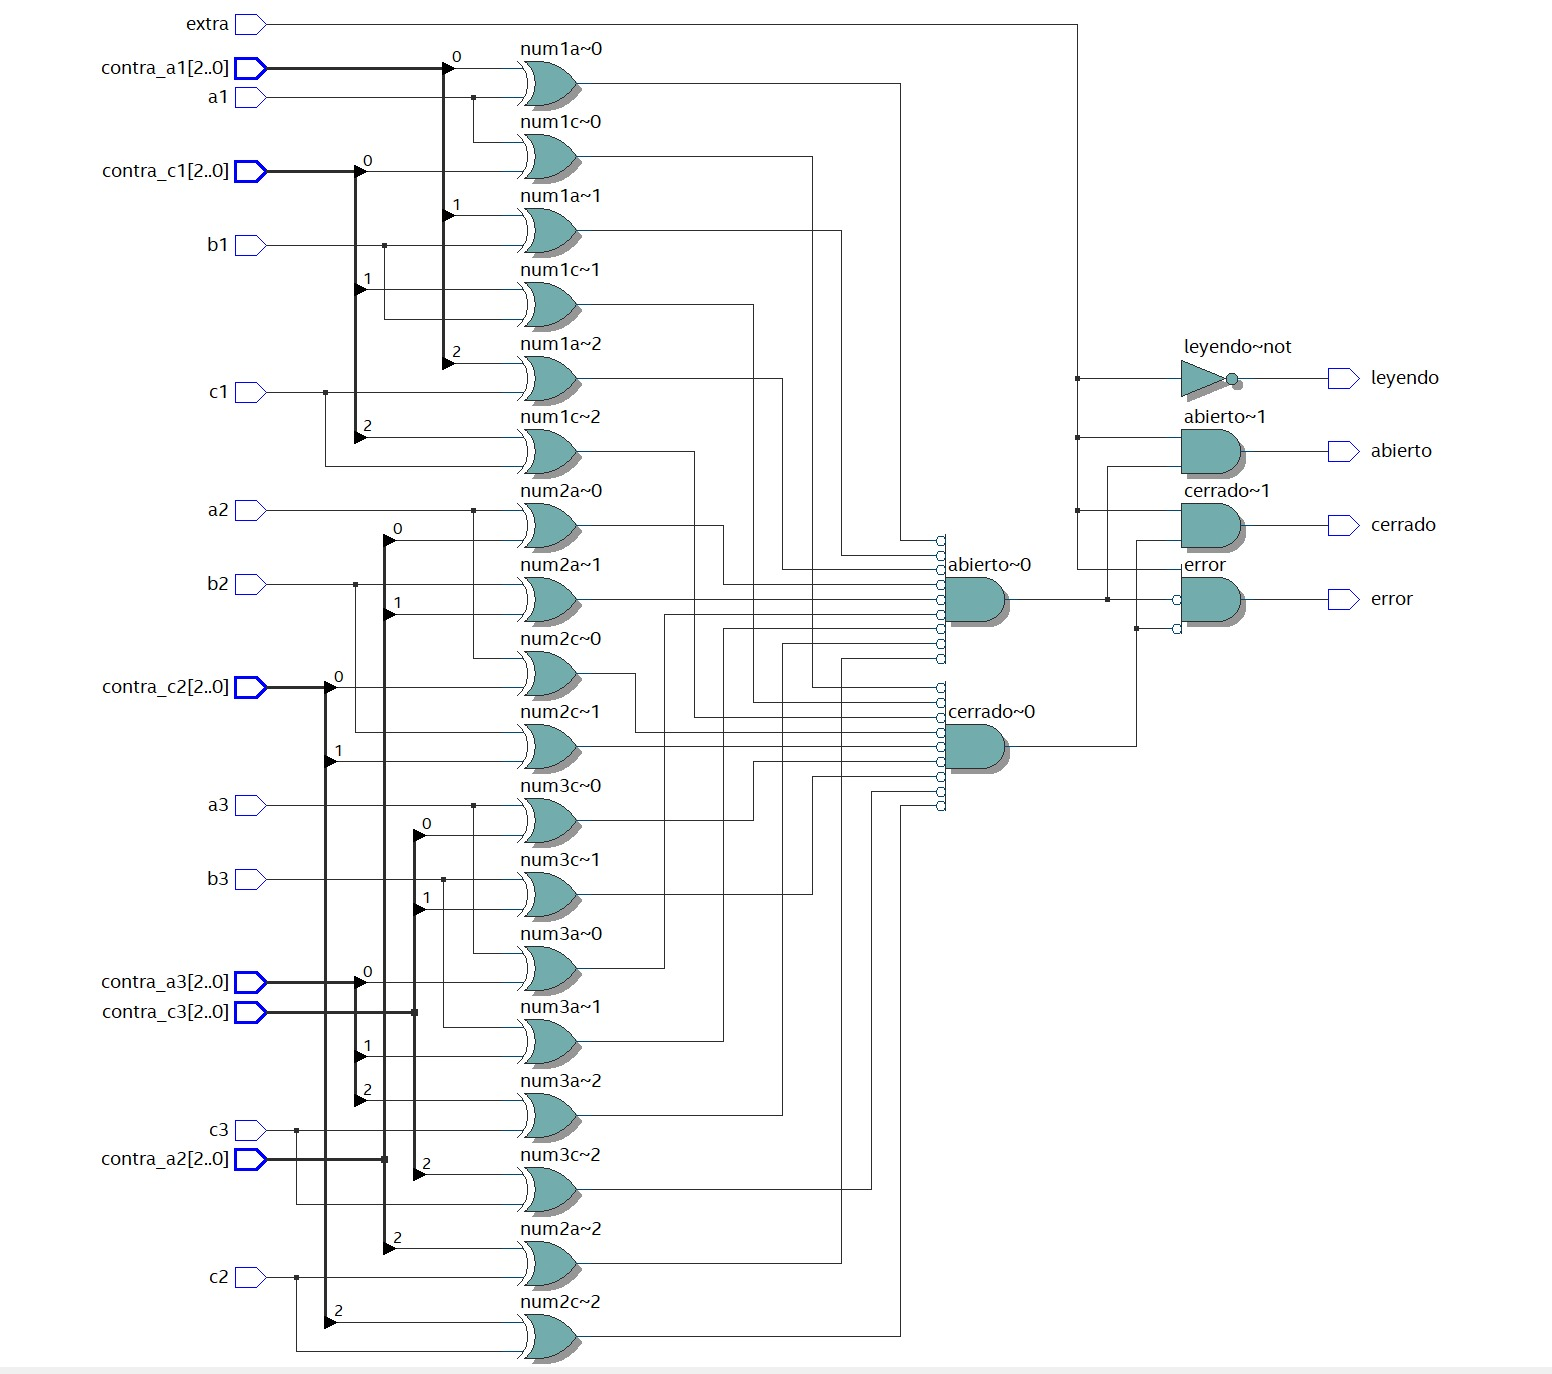
\includegraphics[width=0.95\linewidth]{img/comparador_v1.jpg}
\caption{Primer modelo del verificador: comparaci\'on bit a bit contra referencias configurables
(\emph{contra\_a}, \emph{contra\_c}) mediante XNOR.}
\label{fig:comparador_v1}
\end{figure}

Llamando $A,B,C$ a los 3 bits del primer d\'igito, $D,E,F$ a los
del segundo y $G,H,I$ a los del tercero, en el modelo final el c\'odigo queda ``quemado'' con compuertas NOT en las
entradas correspondientes (Fig.~\ref{fig:comparador_v2}), y la comparaci\'on contra cada c\'odigo
fijo es un solo AND de 9 literales (directos o negados seg\'un el bit valga 1 o 0 en el c\'odigo):
\begin{align}
\mathit{matchC} &= A\,B\,C\,D\,E\,F\,G\,H\,I \quad (\text{seg\'un el patr\'on de }512)\notag\\
\mathit{matchA} &= A\,B\,C\,D\,E\,F\,G\,H\,I \quad (\text{seg\'un el patr\'on de }450)
\label{eq:match}
\end{align}
donde en cada caso los literales que van negados dependen del bit correspondiente de cada c\'odigo
(por eso $matchA$ define qu\'e combinaci\'on abre, y $matchC$ qu\'e combinaci\'on cierra: queda
confirmado en el propio cableado del comparador). De ah\'i salen directo las tres salidas, sin
ning\'un habilitador extra de por medio:
\begin{align}
\mathit{cerrado} &= \mathit{matchC} \notag\\
\mathit{abierto} &= \mathit{matchA} \notag\\
\mathit{error} &= \overline{\mathit{matchC}+\mathit{matchA}}
\end{align}
(\emph{error} se prende cuando la combinaci\'on de switches no calza con ninguno de los dos
c\'odigos).

\begin{figure}[H]
\centering
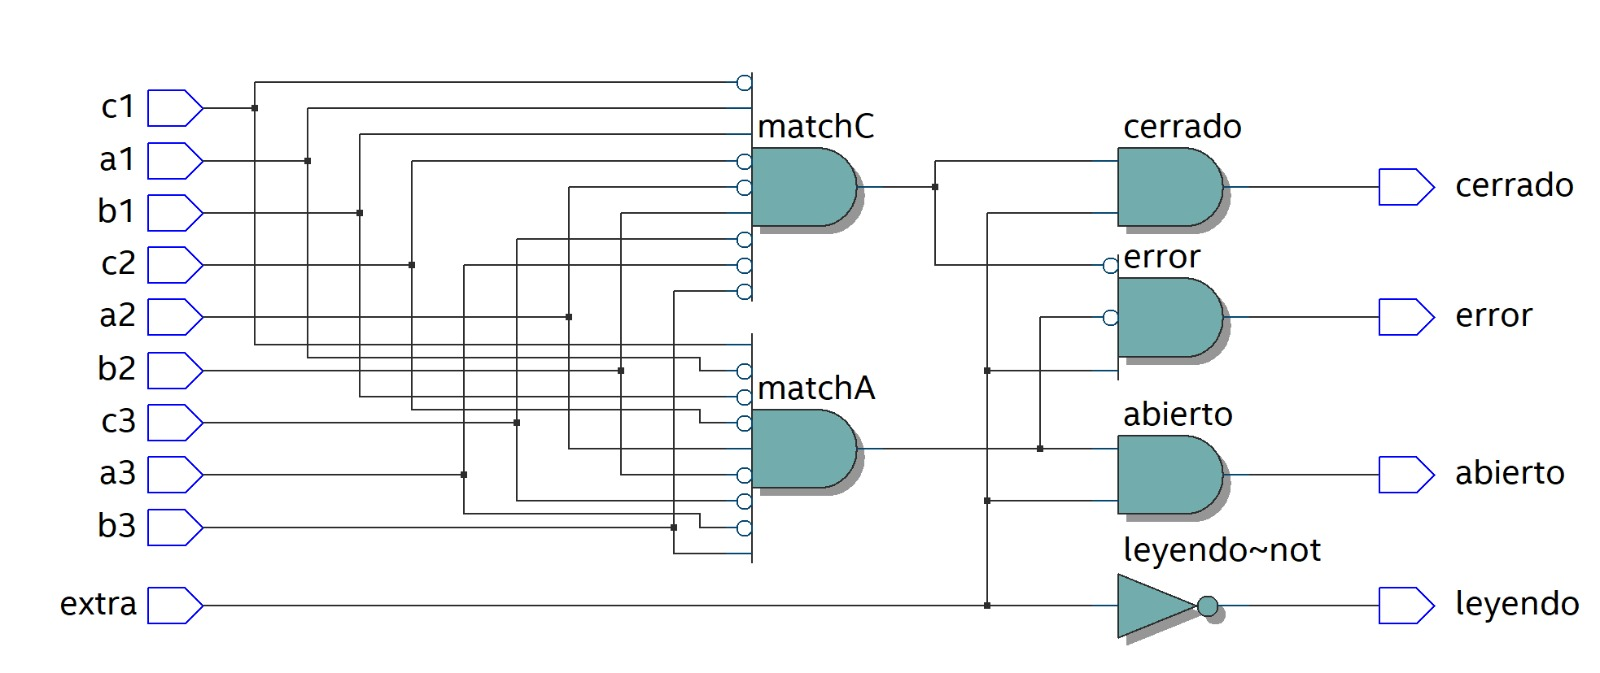
\includegraphics[width=0.95\linewidth]{img/comparador_v2.jpg}
\caption{Comparador de c\'odigo fijo (matchC / matchA) y las salidas cerrado, error, abierto.}
\label{fig:comparador_v2}
\end{figure}

Como la funci\'on completa depende de 9 bits, no tiene caso mostrar la tabla de verdad completa
(512 filas). Alcanza con verla d\'igito por d\'igito: cada bloque de 3 bits solo debe encender en
el valor exacto de ese d\'igito. La Tabla~\ref{tab:digito1} muestra esa comparaci\'on para el primer
d\'igito ($A,B,C$) con los dos patrones usados en el c\'odigo real (\texttt{5} para cerrar,
\texttt{4} para abrir).

\begin{table}[H]
\centering
\caption{Coincidencia del primer d\'igito contra los patrones de cada c\'odigo}
\label{tab:digito1}
\begin{tabular}{ccc|cc}
\toprule
$A$ & $B$ & $C$ & cierra (5) & abre (4)\\
\midrule
0&0&0 & 0&0\\
0&0&1 & 0&0\\
0&1&0 & 0&0\\
0&1&1 & 0&0\\
1&0&0 & 0&1\\
1&0&1 & 1&0\\
1&1&0 & 0&0\\
1&1&1 & 0&0\\
\bottomrule
\end{tabular}
\end{table}

De las 8 combinaciones posibles solo una enciende cada salida, as\'i que el mapa K
(Tabla~\ref{tab:kmap_digito1}) queda con un solo 1 aislado, sin nada que agrupar: la expresi\'on ya
es m\'inima tal como qued\'o cableada, $A\,\overline{B}\,C$ para el patr\'on de cerrar. An\'alogamente,
para el patr\'on de abrir el \'unico 1 cae en $A=1$, $BC=00$, dando $A\,\overline{B}\,\overline{C}$.

\begin{table}[H]
\centering
\caption{Mapa K de la coincidencia del primer d\'igito (patr\'on 5, cerrar)}
\label{tab:kmap_digito1}
\begin{tabular}{c|cccc}
\toprule
$A\backslash BC$ & 00 & 01 & 11 & 10\\
\midrule
0 & 0 & 0 & 0 & 0\\
1 & 0 & 1 & 0 & 0\\
\bottomrule
\end{tabular}
\end{table}

El mismo patr\'on se repite para el segundo d\'igito ($D,E,F$, c\'odigos \texttt{1} para cerrar y
\texttt{5} para abrir, Tabla~\ref{tab:digito2}) y para el tercero ($G,H,I$, c\'odigos \texttt{2} para
cerrar y \texttt{0} para abrir, Tabla~\ref{tab:digito3}): en ambos casos, de las 8 combinaciones
posibles solo una enciende cada salida.

\begin{table}[H]
\centering
\caption{Coincidencia del segundo d\'igito contra los patrones de cada c\'odigo}
\label{tab:digito2}
\begin{tabular}{ccc|cc}
\toprule
$D$ & $E$ & $F$ & cierra (1) & abre (5)\\
\midrule
0&0&0 & 0&0\\
0&0&1 & 1&0\\
0&1&0 & 0&0\\
0&1&1 & 0&0\\
1&0&0 & 0&0\\
1&0&1 & 0&1\\
1&1&0 & 0&0\\
1&1&1 & 0&0\\
\bottomrule
\end{tabular}
\end{table}

\begin{table}[H]
\centering
\caption{Mapa K de la coincidencia del segundo d\'igito (patr\'on 1, cerrar)}
\label{tab:kmap_digito2}
\begin{tabular}{c|cccc}
\toprule
$D\backslash EF$ & 00 & 01 & 11 & 10\\
\midrule
0 & 0 & 1 & 0 & 0\\
1 & 0 & 0 & 0 & 0\\
\bottomrule
\end{tabular}
\end{table}

Otra vez el mapa K de la Tabla~\ref{tab:kmap_digito2} queda con un \'unico 1 en $D=0$, $EF=01$, dando
$\overline{D}\,\overline{E}\,F$; para el patr\'on de abrir el \'unico 1 cae en $D=1$, $EF=01$, dando
$D\,\overline{E}\,F$.

\begin{table}[H]
\centering
\caption{Coincidencia del tercer d\'igito contra los patrones de cada c\'odigo}
\label{tab:digito3}
\begin{tabular}{ccc|cc}
\toprule
$G$ & $H$ & $I$ & cierra (2) & abre (0)\\
\midrule
0&0&0 & 0&1\\
0&0&1 & 0&0\\
0&1&0 & 1&0\\
0&1&1 & 0&0\\
1&0&0 & 0&0\\
1&0&1 & 0&0\\
1&1&0 & 0&0\\
1&1&1 & 0&0\\
\bottomrule
\end{tabular}
\end{table}

\begin{table}[H]
\centering
\caption{Mapa K de la coincidencia del tercer d\'igito (patr\'on 2, cerrar)}
\label{tab:kmap_digito3}
\begin{tabular}{c|cccc}
\toprule
$G\backslash HI$ & 00 & 01 & 11 & 10\\
\midrule
0 & 0 & 0 & 0 & 1\\
1 & 0 & 0 & 0 & 0\\
\bottomrule
\end{tabular}
\end{table}

El mapa K de la Tabla~\ref{tab:kmap_digito3} vuelve a quedar con un \'unico 1, en $G=0$, $HI=10$,
dando $\overline{G}\,H\,\overline{I}$; para el patr\'on de abrir el \'unico 1 cae en $G=0$, $HI=00$,
dando $\overline{G}\,\overline{H}\,\overline{I}$.

Como los tres bloques de 3 bits ($A,B,C$; $D,E,F$; $G,H,I$) usan variables completamente
independientes entre s\'i, y cada uno ya es una funci\'on de un solo minit\'ermino --- es decir, ya
m\'inima, sin ning\'un otro 1 adyacente con el cual agruparse en su propio mapa K ---, el producto
AND de los tres t\'erminos tampoco se puede reducir m\'as: ninguna ley de \'algebra booleana
(absorci\'on, consenso, idempotencia) permite simplificar un AND de literales que pertenecen a
variables distintas. As\'i, $matchC$ y $matchA$ (Ecuaci\'on~\ref{eq:match}) ya son la expresi\'on
m\'inima de todo el comparador, sin necesidad de construir (ni de que exista) un mapa K de 9
variables.

Se simul\'o antes de armar nada f\'isico, y se confirm\'o que abierto y cerrado nunca se prenden al
mismo tiempo (por construcci\'on, matchA y matchC no pueden dar 1 a la vez). Este es el circuito
que se termin\'o implementando f\'isicamente.

\section{15 de septiembre --- decodificador de 7 segmentos}
\textbf{Objetivo:} traducir las tres salidas del comparador (abierto/cerrado/error) a los
segmentos $a$--$g$ del display, mostrando A (abriendo), C (cerrando) o E (clave inv\'alida).

Se hizo la tabla de verdad con 3 entradas: $A$=\emph{abierto}, $B$=\emph{cerrado} y
$C$=\emph{error}. Por c\'omo qued\'o armado el comparador, exactamente una de las tres siempre est\'a
en 1 (nunca las tres en 0, ni dos a la vez), as\'i que las otras 5 combinaciones de $(A,B,C)$ no
pueden pasar y se dejan como no importa ($\times$), ver Tabla~\ref{tab:seg}.

\begin{table}[H]
\centering
\caption{Tabla de verdad del decodificador de 7 segmentos}
\label{tab:seg}
\begin{tabular}{ccc|ccccccc}
\toprule
$A$ & $B$ & $C$ & $a$ & $b$ & $c$ & $d$ & $e$ & $f$ & $g$\\
\midrule
0&0&0 & $\times$&$\times$&$\times$&$\times$&$\times$&$\times$&$\times$\\
1&0&0 & 1&1&1&0&1&1&1\\
0&1&0 & 1&0&0&1&1&1&0\\
0&0&1 & 1&0&0&1&1&1&1\\
1&1&0 & $\times$&$\times$&$\times$&$\times$&$\times$&$\times$&$\times$\\
1&0&1 & $\times$&$\times$&$\times$&$\times$&$\times$&$\times$&$\times$\\
0&1&1 & $\times$&$\times$&$\times$&$\times$&$\times$&$\times$&$\times$\\
1&1&1 & $\times$&$\times$&$\times$&$\times$&$\times$&$\times$&$\times$\\
\bottomrule
\end{tabular}
\end{table}

Un primer borrador (sin reducir, Fig.~\ref{fig:seg7}) simplemente sac\'o $seg_d$ y $seg_g$ como un
OR directo de $A$/$B$/$C$. Por ejemplo, tomando solo los minit\'erminos donde el segmento debe
encender (sin usar todav\'ia los $\times$), esos dos quedaban as\'i antes de reducir:
\begin{align}
seg_d\ (\text{antes}) &= \overline{A}\,B\,\overline{C} + \overline{A}\,\overline{B}\,C\\
seg_g\ (\text{antes}) &= A\,\overline{B}\,\overline{C} + \overline{A}\,\overline{B}\,C
\end{align}
Al meter los $\times$ en el mapa K esas expresiones se reducen mucho:
\begin{align}
seg_a &= 1 & seg_e &= 1\notag\\
seg_b &= A & seg_f &= 1\notag\\
seg_c &= A & seg_g &= \overline{B}\notag\\
seg_d &= \overline{A} & &
\end{align}
Es decir, $a$, $e$ y $f$ quedan siempre encendidos (no hace falta ni una compuerta para ellos), y
$b$, $c$, $d$, $g$ terminan dependiendo de una sola variable cada uno, gracias a que las
combinaciones imposibles se pudieron usar a favor en el mapa K. Esta reducci\'on tambi\'en se
corri\'o por un modelo de IA junto con el mapa K para confirmar que no quedara ning\'un t\'ermino
de m\'as, y coincidi\'o.

\begin{figure}[H]
\centering
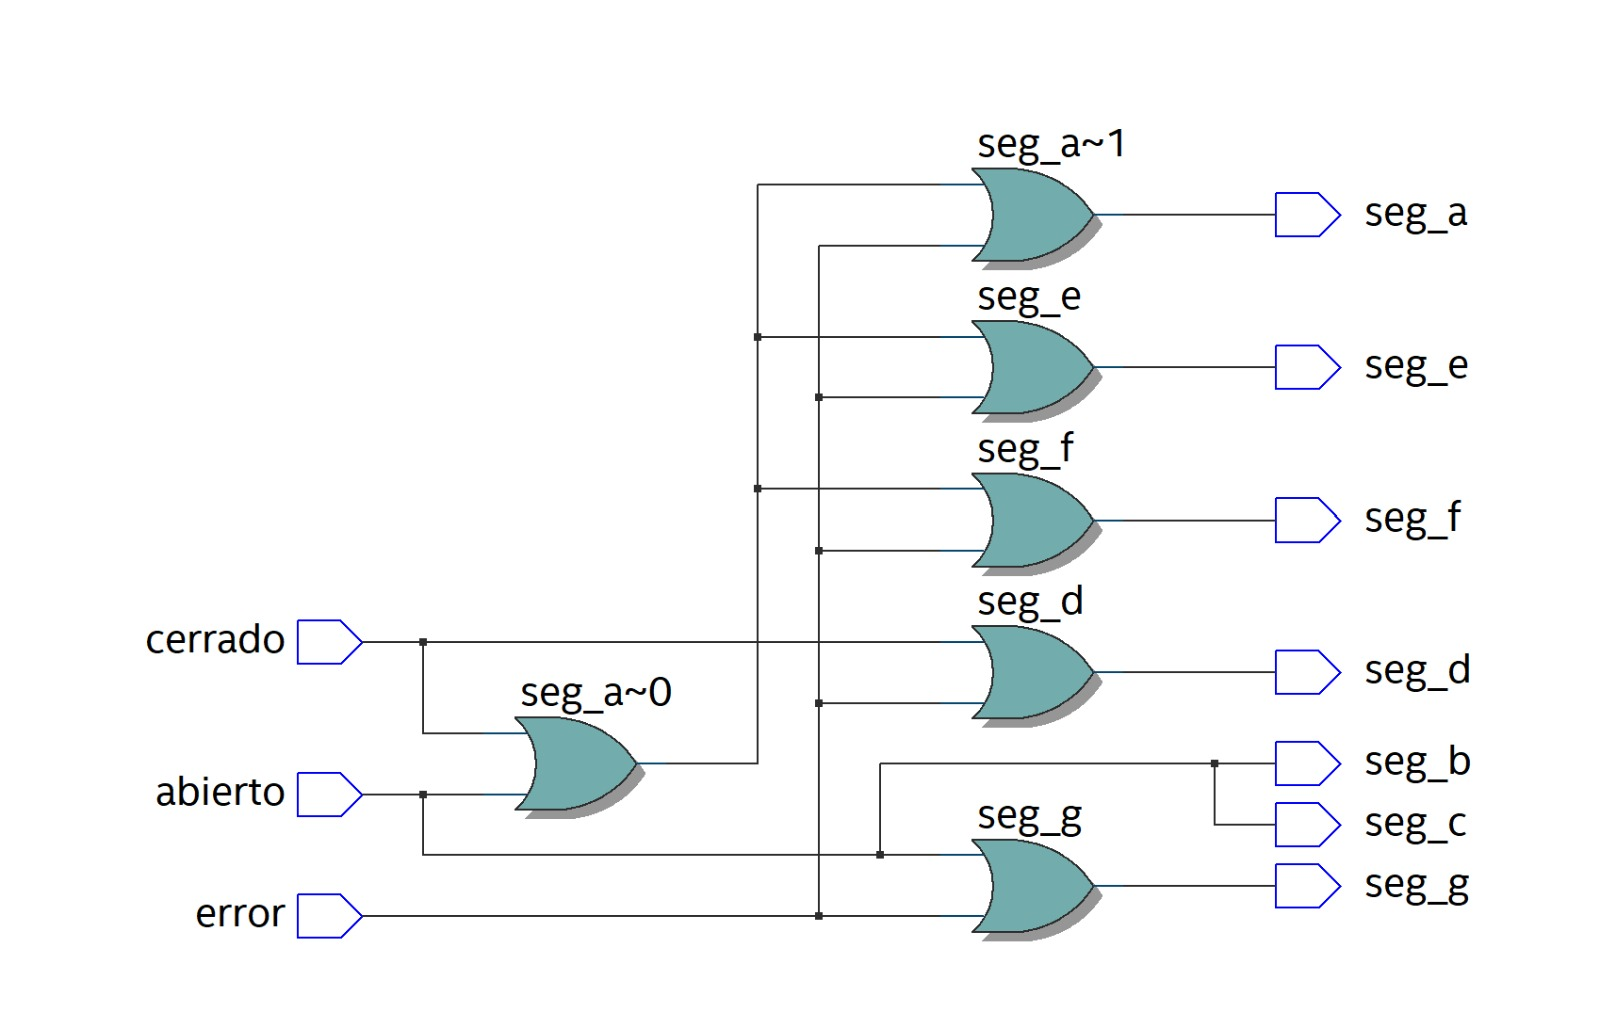
\includegraphics[width=0.95\linewidth]{img/decodificador_7seg.jpg}
\caption{Borrador inicial sin reducir del decodificador de 7 segmentos.}
\label{fig:seg7}
\end{figure}

\FloatBarrier

\section{16 de septiembre --- integraci\'on y pruebas}
\textbf{Objetivo:} armar en protoboard el verificador de contrase\~na junto con el decodificador
de 7 segmentos ya reducido, y probar que funcione con los dos c\'odigos.

Se mont\'o todo en dos protoboards acopladas (Fig.~\ref{fig:breadboard}): la de la izquierda tiene
los dos DIP-switch con el c\'odigo puesto y el circuito integrado del comparador; la de la derecha
tiene el decodificador de 7 segmentos y el display de salida. Cada banco de switches se conecta al positivo a trav\'es de una resistencia de pull-up de
10\,k$\Omega$, de forma que la entrada quede en alto cuando el switch est\'a abierto y se vaya a
bajo solo cuando se cierra; son las dos resistencias que se ven en la esquina superior izquierda de
la protoboard.

\begin{figure}[H]
\centering
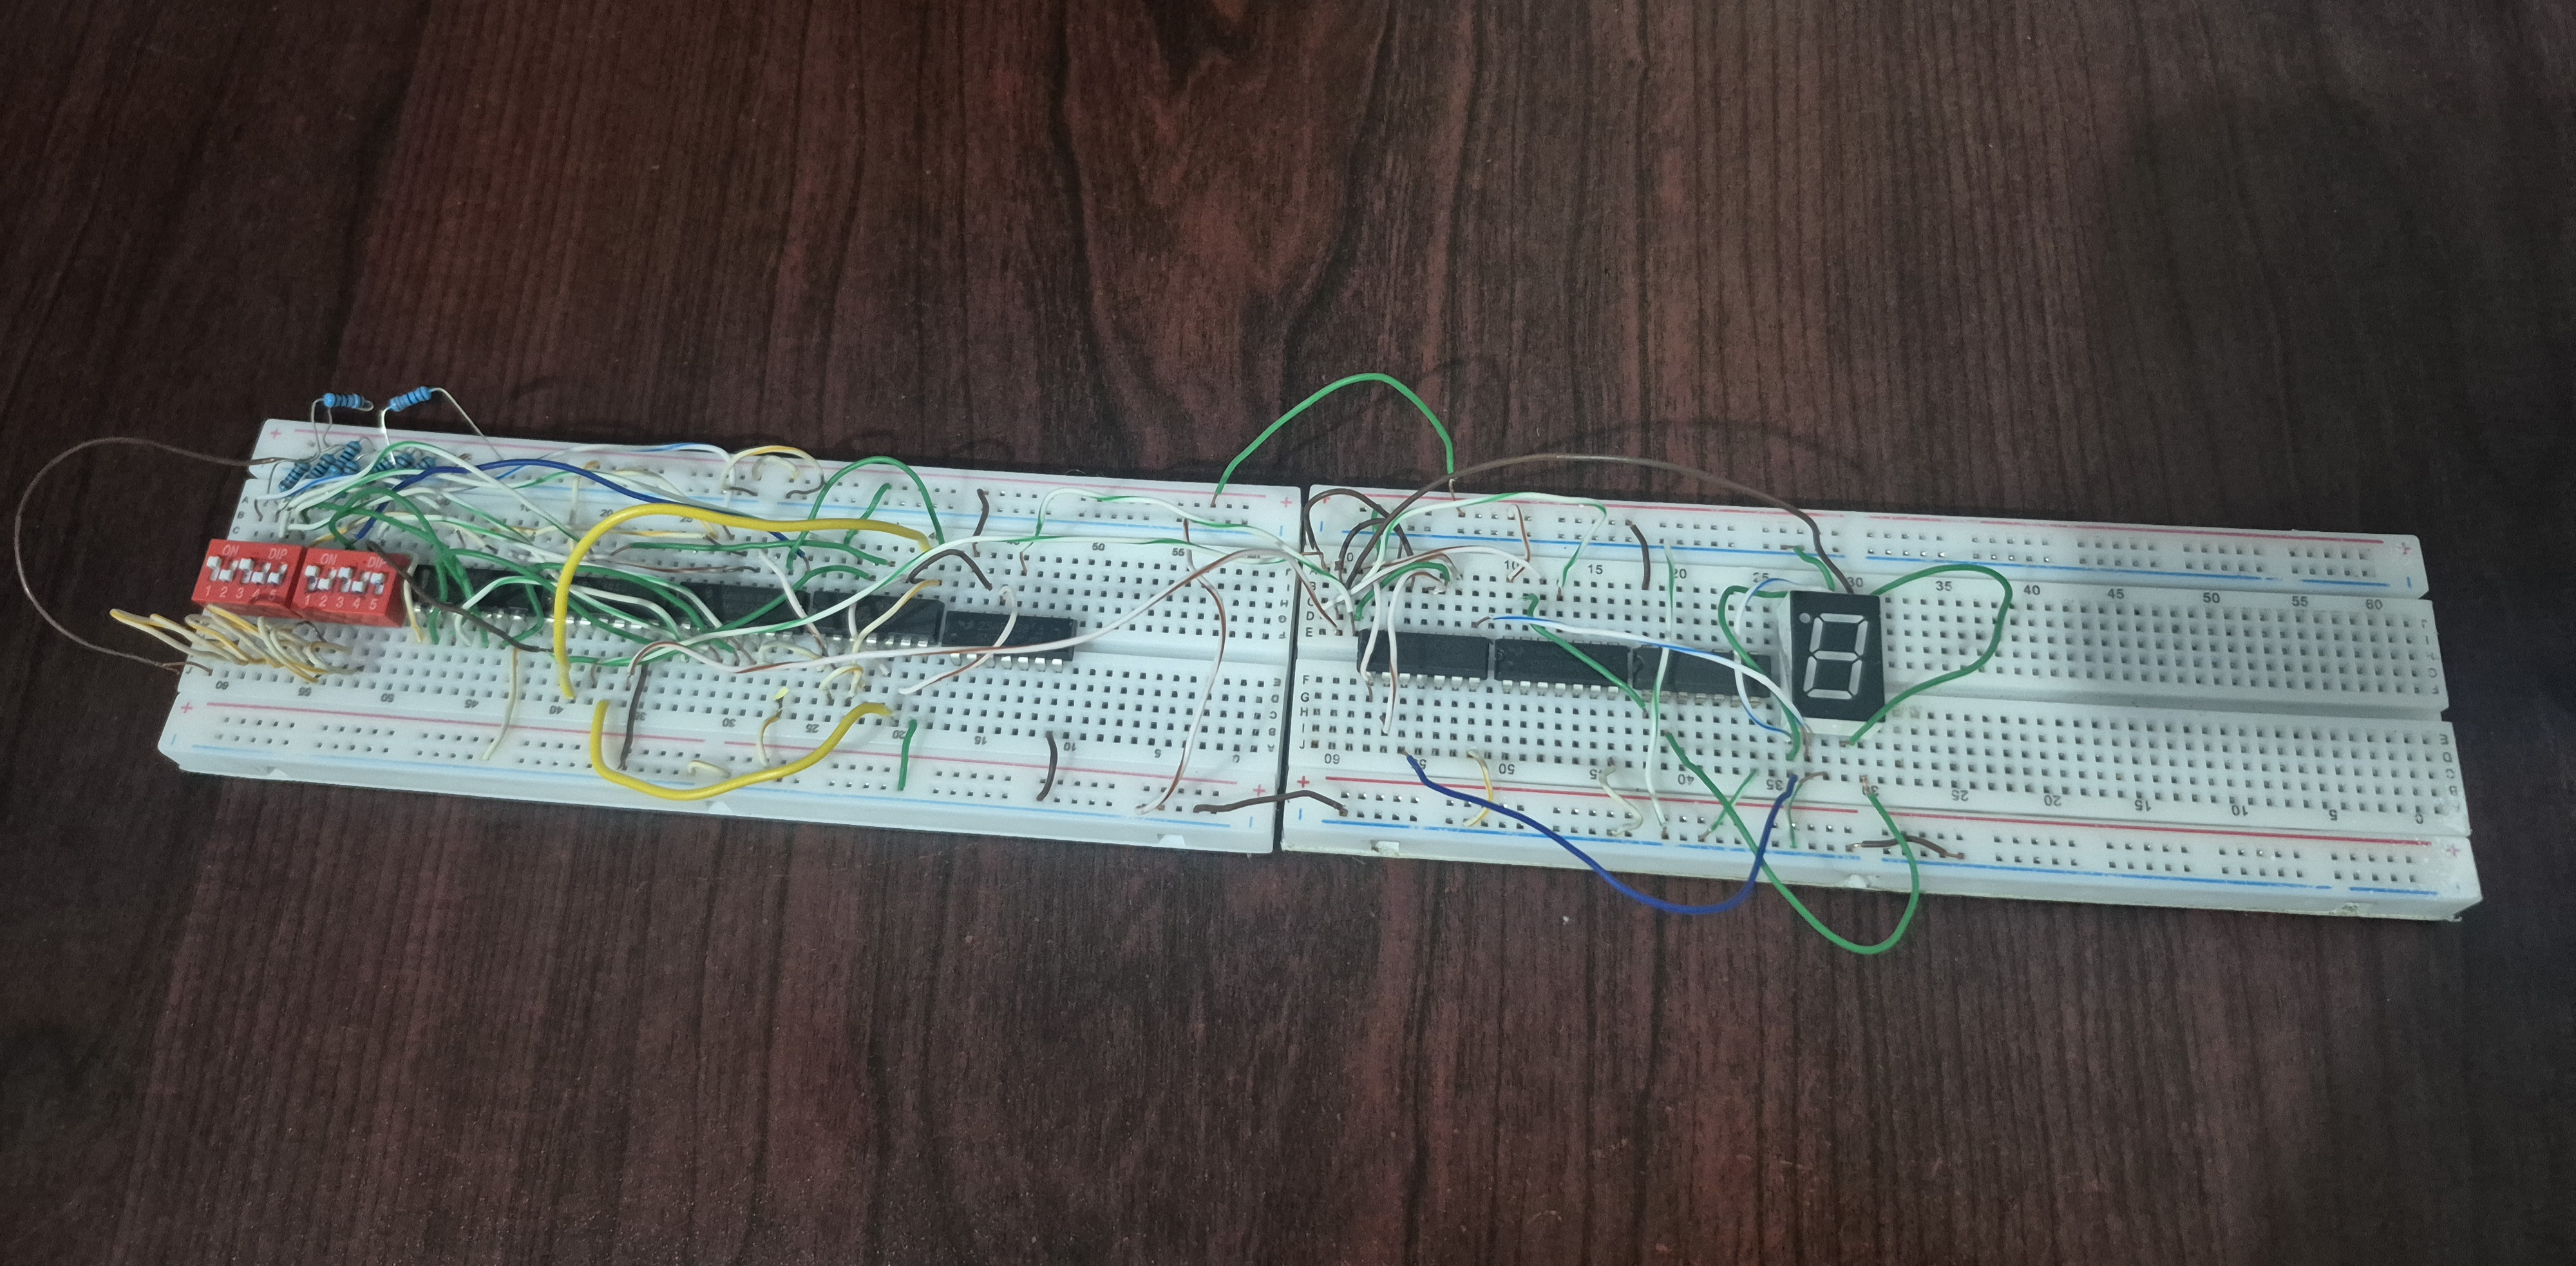
\includegraphics[width=0.95\linewidth]{img/breadboard.jpg}
\caption{Verificador de contrase\~na (izquierda) y decodificador de 7 segmentos (derecha) ya
integrados en protoboard.}
\label{fig:breadboard}
\end{figure}

Se prob\'o con el c\'odigo \texttt{450} (abre, muestra ``A''), con \texttt{512} (cierra, muestra
``C'') y con una combinaci\'on que no coincide con ninguno (muestra ``E''). En la primera prueba,
antes de terminar de cablear las tres salidas del comparador hacia el decodificador, el display
qued\'o mostrando todos los segmentos prendidos (como un ``8''), lo que sirvi\'o para confirmar que
el display en s\'i estaba bien y que el problema era ese cableado, no los circuitos integrados. Ya
corregido, los tres casos funcionaron bien.

\end{document}